\documentclass[11pt,letterpaper]{article}
\usepackage[utf8x]{inputenc}
\usepackage[T1]{fontenc}
\usepackage{amsmath}
\usepackage{amssymb}
\usepackage{graphicx}
\graphicspath{{../img/}}
\usepackage[spanish]{babel}

\title{Simulación Estocástica\\Taller 3}
\author{Jesid Mauricio Mejía Castro}

\begin{document}
	\maketitle
	
	\section{Cadenas de Markov de Tiempo Discreto}	
	\begin{itemize}
		\item[a)] Este problema puede modelarse como una CMTD si su conjunto de estados se define como el número de pruebas exitosas en el instante $n$, es decir $S = \{1,2,3, \ldots\}$. De manera que su matriz de probabilidad de transición estaría definida por 
		
		\[
		\mathbb{P} = 
		\left( 
		\begin{matrix}
			0.5 & 0.5 & 0 & 0 \\
			0 & 0.5 & 0.5 & 0 \\
			0 & 0 & 0.2 & 0.8 \\
			0.5 & 0 & 0 & 0.5
		\end{matrix}
		\right) \text{.}
		\]
		
		Por último, podemos ver una representación gráfica de la cadena de Markov en la Figura \ref{fig:1}.
		
		\begin{figure}[h!]
			\centering
			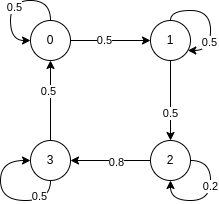
\includegraphics[width=0.5\linewidth]{../img/cmtd.png}
			\caption{Cadena de Markov de Tiempo Discreto.}
			\label{fig:1}
		\end{figure}
	
		%\newpage
		
		\item[b)] Uilizando el paquete \texttt{markovchain} y su función \texttt{steadyStates()} se obtiene el siguiente resultado resultado (consultar archivo \texttt{p1.r}):
		
		\begin{verbatim}
			                  0         1         2         3
			     [1,] 0.2758621 0.2758621 0.1724138 0.2758621
		\end{verbatim}
	
		Esto entra en resonancia con el hecho de que la cadena no contiene estados \textit{absorbentes}.
		
		\item[c)] Al realizar una simulación de 1000 pasos sobre la cadena de Markov se obitenen la proporción para la los estados:
		
		\begin{verbatim}
			[0] 0.259
			[1] 0.288
			[2] 0.167
			[3] 0.286
		\end{verbatim}
		
		De donde conluimos que la proporción de estados exitosos es $0.286+0.167+0.286=0.739$.
	\end{itemize}
	
	%\newpage
	
	\section{Ruido blanco con distribución t-student y caminata aleatoria}
	
	\begin{itemize}
		\item[a)] Observe que 
		
		\[
		E[e_t] = E \left[ \sqrt{\frac{\nu - 2}{\nu}}X \right] 
		= \sqrt{\frac{\nu - 2}{\nu}} E[X] \text{.}
		\]
		
		Dado que $E[X] = 0$, se sigue que $E[e_t] = 0$.
		
		Por otro lado, aplicando las propiedades de la varianza, se obtiene
		
		\[
		V(e_t) = V\left( \sqrt{\frac{\nu - 2}{\nu}}X \right) 
		= \frac{\nu - 2}{\nu}V(X) = \frac{\nu - 2}{\nu} \frac{\nu}{\nu - 2} = 1 \text{.}
		\]
		
		\item[b)] Con $10^4$ realizaciones del ruido blanco \textit{t-student}, se obtiene que el mínimo valor es -24,77254 y el máximo valor es 20.16167. Mientras que para el ruido blanco normal estándar se obtiene que el mínimo valor es -3.801588 y el máximo es 4.111151.
		
		\item[c)] El código de las simulaciones puede encontrarse en el archivo \texttt{p2.R}. La Figura \ref{fig:2} muestra la gráfica del ruido blanco \textit{t-student} mientras que la Figura \ref{fig:3} muestra el ruido blanco normal estándar.
		
		\begin{figure}[!t]
			\centering
			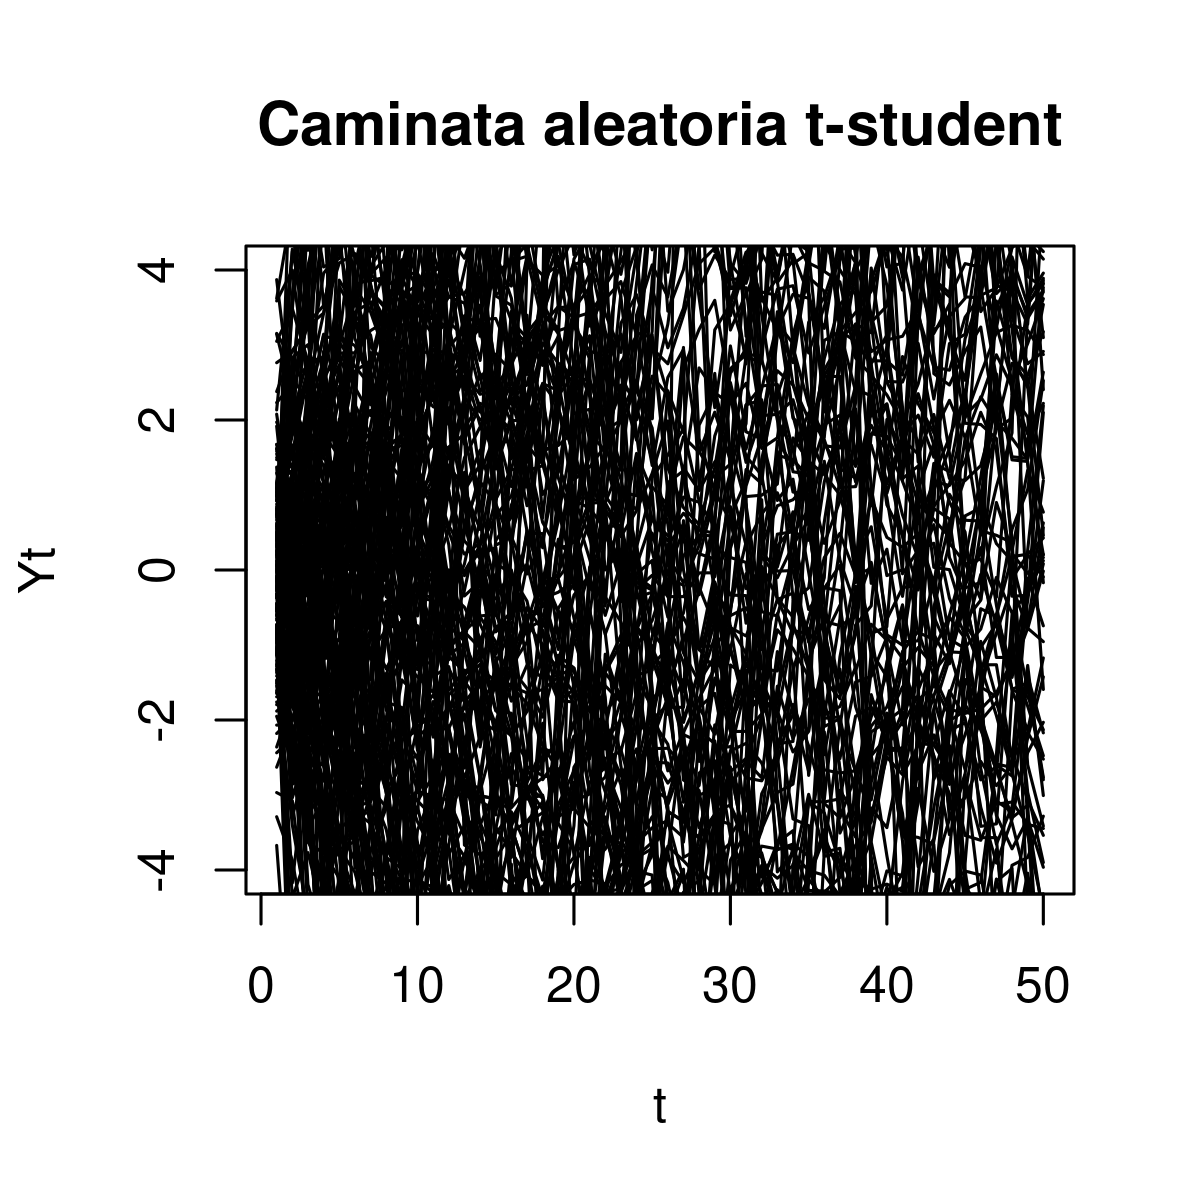
\includegraphics[width=0.6\linewidth]{../img/rb_et.png}
			\caption{Ruido blanco \textit{t-student}}
			\label{fig:2}
		\end{figure}
		
		\begin{figure}[!t]
			\centering
			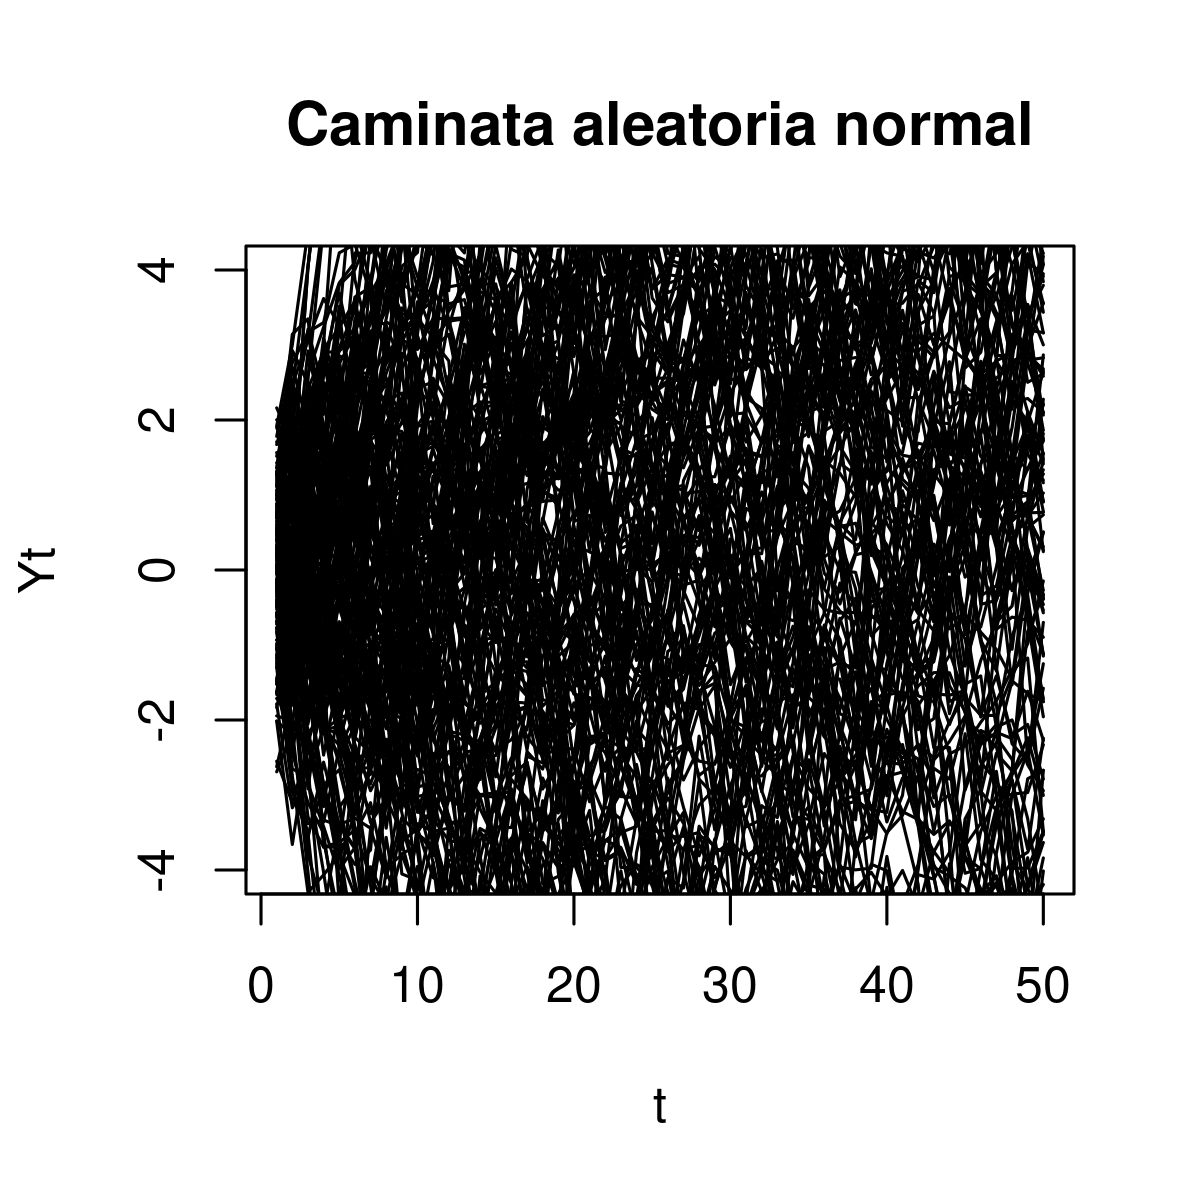
\includegraphics[width=0.6\linewidth]{../img/rb_enorm.png}
			\caption{Ruido blanco normal estándar}
			\label{fig:3}
		\end{figure}
		
	\end{itemize}
	
	\section{Series de tiempo}
	El conjunto de datos \texttt{wages} contiene valores mensuales del salario promedio por hora (en dólares) para trabajadores en la industria textil de EE.UU. desde julio de 1981 hasta junio de 1987.
	
	\begin{itemize}
		\item[a)] Muestre e interprete la gráfica de serie de tiempo de estos datos.
		\item[b)] Utilize mínimos cuadrados para ajustar linealmente esta serie de tiempo. Interprete la salida de la regresión. Guarde los residuales estandarizados para un análisis posterior.
		\item[c)] Construya e interprete la gráfica de serie de tiempo de los residuales estandarizados de la parte b.
		\item[d)] Utilize mínimos cuadrados para ajustar cuadraticamente esta serie de tiempo. Interprete la salida de la regresión. Guarde los residuales estandarizados para un análisis posterior.
		\item[e)] Construya e interprete la gráfica de serie de tiempo de los residuales estandarizados de la parte d.
	\end{itemize}

	\textit{Solución:}
	
	\begin{itemize}
		\item[a)] La Figura \ref{fig:4} muestra la gráfica de serie de tiempo del conjunto de datos. Este aumento en los salarios en función del tiempo es esperado pues muy posiblemente está asociado a los aumentos normales en la inflación y el aumento de los precios de bienes y servicios que ocurre en todas las economias.
		
		\begin{figure}[!h]
			\centering
			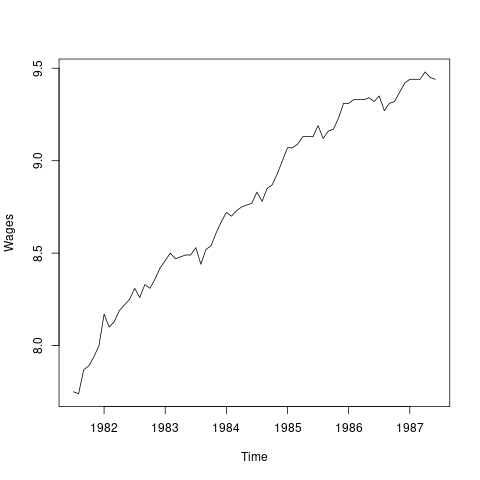
\includegraphics[width=0.6\linewidth]{../img/wages_plot.png}
			\caption{Serie de tiempo para \texttt{wages}}
			\label{fig:4}
		\end{figure}
		
		\item[b)] Al ajustar la serie de tiempo con un modelo lineal, se obtiene el siguiente resumen:
		
		\begin{verbatim}
			Call:
			lm(formula = wages ~ w)
			
			Residuals:
			Min       1Q   Median       3Q      Max 
			-0.23828 -0.04981  0.01942  0.05845  0.13136 
			
			Coefficients:
			Estimate Std. Error t value Pr(>|t|)    
			(Intercept) -5.490e+02  1.115e+01  -49.24   <2e-16 ***
			w            2.811e-01  5.618e-03   50.03   <2e-16 ***
			---
			Signif. codes:  0 ‘***’ 0.001 ‘**’ 0.01 ‘*’ 0.05 ‘.’ 0.1 ‘ ’ 1
			
			Residual standard error: 0.08257 on 70 degrees of freedom
			Multiple R-squared:  0.9728,    Adjusted R-squared:  0.9724 
			F-statistic:  2503 on 1 and 70 DF,  p-value: < 2.2e-16
		\end{verbatim}
		
		\item[c)] La Figura \ref{fig:5} meustra la gráfica de los residuales para la serie de tiempo ajustada con el modelo lineal.
		
		\begin{figure}[!h]
			\centering
			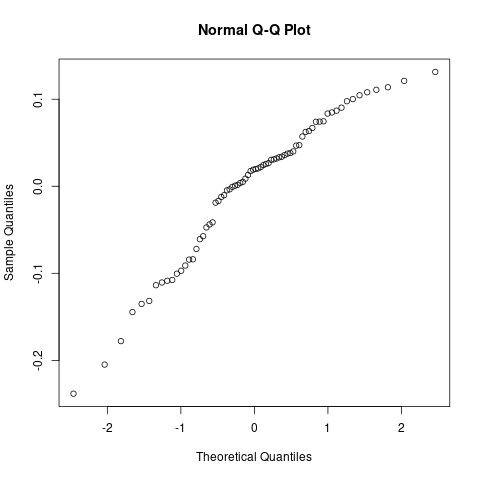
\includegraphics[width=0.6\linewidth]{../img/qqnorm_linear.png}
			\caption{Gráfica de residuales estandarizados para ajuste lineal.}
			\label{fig:5}
		\end{figure}
		
		\item[d)] Al ajustar la serie de tiempo con un modelo cuadrático, se obtiene el siguiente resumen:
		
		\begin{verbatim}
			Call:
			lm(formula = wages ~ w + I(w^2))
			
			Residuals:
			Min        1Q    Median        3Q       Max 
			-0.148318 -0.041440  0.001563  0.050089  0.139839 
			
			Coefficients:
			Estimate Std. Error t value Pr(>|t|)    
			(Intercept) -8.495e+04  1.019e+04  -8.336 4.87e-12 ***
			w            8.534e+01  1.027e+01   8.309 5.44e-12 ***
			I(w^2)      -2.143e-02  2.588e-03  -8.282 6.10e-12 ***
			---
			Signif. codes:  0 ‘***’ 0.001 ‘**’ 0.01 ‘*’ 0.05 ‘.’ 0.1 ‘ ’ 1
			
			Residual standard error: 0.05889 on 69 degrees of freedom
			Multiple R-squared:  0.9864,    Adjusted R-squared:  0.986 
			F-statistic:  2494 on 2 and 69 DF,  p-value: < 2.2e-16
		\end{verbatim}
		
		\item[e)] La Figura \ref{fig:6} meustra la gráfica de los residuales para la serie de tiempo ajustada con el modelo lineal. Al compararlo con el ajuste lineal, no se evidencia una diferencia decisiva entre los dos modelos. Sin embargo, basandonos en $r^2$ se ve que el modelo cuadratico explica mejor la variación. Esto lo confirma las graficas \ref{fig:7} y \ref{fig:8} de los residuales contra el ajuste.
		
		\begin{figure}[!h]
			\centering
			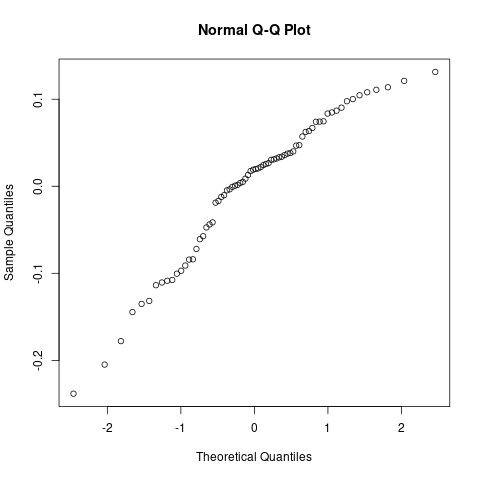
\includegraphics[width=0.6\linewidth]{../img/qqnorm_linear.png}
			\caption{Gráfica de residuales estandarizados para el ajuste cuadrático.}
			\label{fig:6}
		\end{figure}
	
		\begin{figure}[!h]
			\centering
			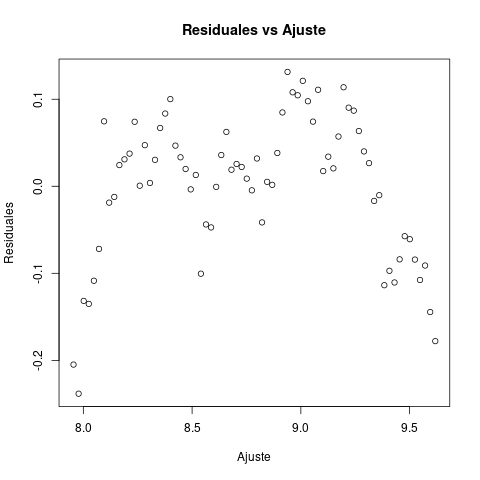
\includegraphics[width=0.6\linewidth]{../img/res_linear.png}
			\caption{Gráfica de residuales contra ajuste para el modelo lineal.}
			\label{fig:7}
		\end{figure}
	
		\begin{figure}[!h]
			\centering
			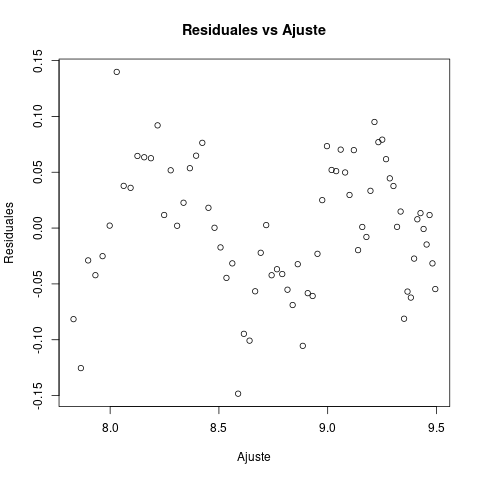
\includegraphics[width=0.6\linewidth]{../img/res_cuadr.png}
			\caption{Gráfica de residuales contra ajuste para el modelo cuadrático.}
			\label{fig:8}
		\end{figure}
	\end{itemize}
	
\end{document}